\documentclass[tikz,border=2pt]{standalone}
% Shared Figure architecture visual system for all four main-text figures.
\usepackage[T1]{fontenc}
\usepackage{charter}
\usepackage[scaled=0.90]{helvet}
\usepackage{amsmath,amssymb}
\renewcommand{\Pr}{\mathbb{P}}
\usepackage{xcolor}
\usepackage{tikz}
\usepackage{pgfplots}
\pgfplotsset{compat=1.18}
\usetikzlibrary{arrows.meta,calc,positioning,fit,decorations.pathreplacing,shapes.geometric,backgrounds}
\definecolor{figNavy}{RGB}{0,63,92}
\definecolor{figBlue}{RGB}{0,101,165}
\definecolor{figSky}{RGB}{226,241,249}
\definecolor{figTeal}{RGB}{0,125,112}
\definecolor{figMint}{RGB}{224,243,239}
\definecolor{figOrange}{RGB}{222,102,35}
\definecolor{figPeach}{RGB}{252,235,224}
\definecolor{figRed}{RGB}{145,43,55}
\definecolor{figInk}{RGB}{35,45,51}
\definecolor{figGray}{RGB}{103,115,123}
\definecolor{figRule}{RGB}{194,202,208}
\definecolor{figPale}{RGB}{248,250,251}
\definecolor{figWhite}{RGB}{255,255,255}
\tikzset{
  figpanel/.style={draw=figRule,line width=0.55pt,rounded corners=2.4pt,fill=figWhite},
  figtag/.style={circle,fill=figBlue,text=figWhite,minimum size=4.3mm,inner sep=0pt,font=\sffamily\bfseries\fontsize{7.5}{8}\selectfont},
  figtitle/.style={font=\sffamily\bfseries\fontsize{8.5}{10}\selectfont,text=figNavy,anchor=west},
  figsubtitle/.style={font=\sffamily\fontsize{6.8}{8}\selectfont,text=figGray,align=left},
  figbody/.style={font=\sffamily\fontsize{7}{8.4}\selectfont,text=figInk,align=center},
  figsmall/.style={font=\sffamily\fontsize{6.2}{7.4}\selectfont,text=figGray,align=center},
  figmath/.style={font=\fontsize{7.4}{8.8}\selectfont,text=figInk,align=center},
  figflow/.style={-{Stealth[length=2.0mm,width=1.4mm]},draw=figBlue,line width=0.85pt},
  figflowgray/.style={-{Stealth[length=1.8mm,width=1.25mm]},draw=figGray,line width=0.75pt},
  figfloworange/.style={-{Stealth[length=2.0mm,width=1.4mm]},draw=figOrange,line width=0.85pt},
  figbluebox/.style={draw=figBlue,line width=0.65pt,fill=figSky,rounded corners=2.2pt},
  figorangebox/.style={draw=figOrange,line width=0.65pt,fill=figPeach,rounded corners=2.2pt},
  figtealbox/.style={draw=figTeal,line width=0.65pt,fill=figMint,rounded corners=2.2pt},
  figgraybox/.style={draw=figRule,line width=0.6pt,fill=figPale,rounded corners=2.2pt},
}
\newcommand{\PanelHeading}[4]{%
  \node[figtag] at (#1,#2) {#3};%
  \node[figtitle] at ({#1+0.32},#2) {#4};%
}

\begin{document}
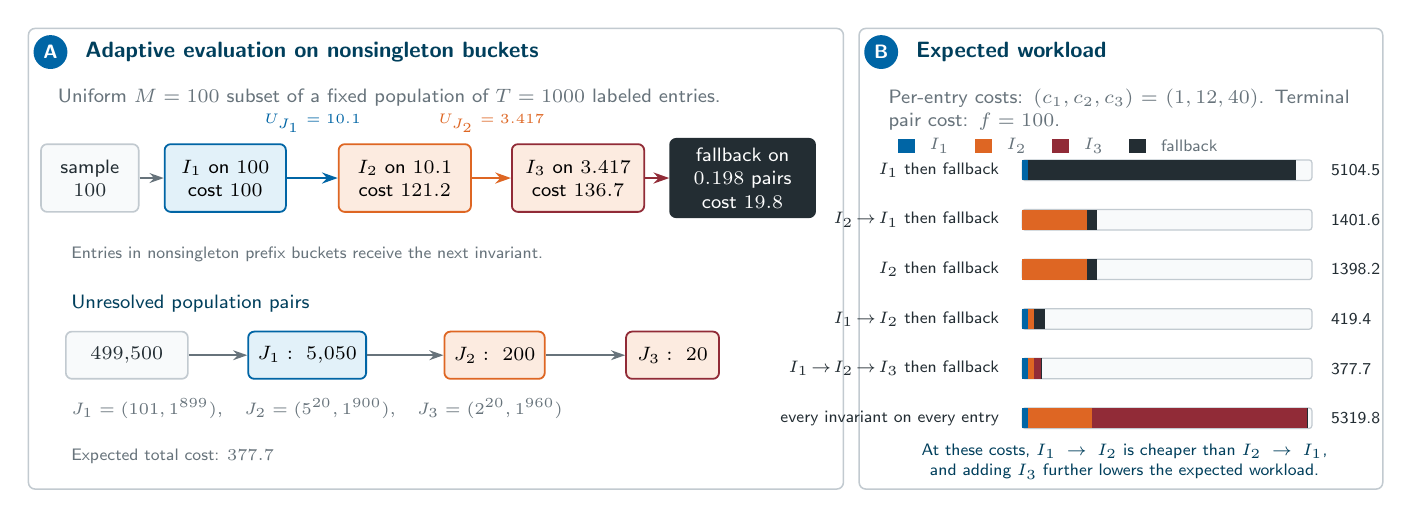
\begin{tikzpicture}[x=1cm,y=1cm]
\tikzset{
  figstageblue/.style={draw=figBlue,line width=0.65pt,fill=figSky,text=black,rounded corners=2.2pt},
  figstageorange/.style={draw=figOrange,line width=0.65pt,fill=figPeach,text=black,rounded corners=2.2pt},
  figstagered/.style={draw=figRed,line width=0.65pt,fill=figPeach,text=black,rounded corners=2.2pt},
  figfallback/.style={draw=figInk,line width=0.65pt,fill=figInk,text=figWhite,rounded corners=2.2pt},
  figflowred/.style={-{Stealth[length=2.0mm,width=1.4mm]},draw=figRed,line width=0.85pt},
}
\draw[figpanel] (0,0) rectangle (10.35,5.85);
\draw[figpanel] (10.55,0) rectangle (17.20,5.85);

% Panel A: flow.
\PanelHeading{0.28}{5.55}{A}{Adaptive evaluation on nonsingleton buckets}
\node[figsubtitle,anchor=north west,text width=9.45cm] at (0.25,5.20)
  {Uniform $M=100$ subset of a fixed population of $T=1000$ labeled entries.};

\node[figgraybox,minimum width=1.24cm,minimum height=0.86cm,figbody] (sample) at (0.78,3.95) {sample\\$100$};
\node[figbody,figstageblue,minimum width=1.54cm,minimum height=0.86cm] (Ione) at (2.50,3.95) {$I_1$ on $100$\\cost $100$};
\node[figbody,figstageorange,minimum width=1.68cm,minimum height=0.86cm] (Itwo) at (4.78,3.95) {$I_2$ on $10.1$\\cost $121.2$};
\node[figbody,figstagered,minimum width=1.68cm,minimum height=0.86cm] (Ithree) at (6.98,3.95) {$I_3$ on $3.417$\\cost $136.7$};
\node[figbody,figfallback,minimum width=1.84cm,minimum height=0.86cm] (fallback) at (9.07,3.95) {fallback on\\$0.198$ pairs\\cost $19.8$};
\draw[figflowgray] (sample.east) -- (Ione.west);
\draw[figflow] (Ione.east) -- (Itwo.west);
\draw[figfloworange] (Itwo.east) -- (Ithree.west);
\draw[figflowred] (Ithree.east) -- (fallback.west);
\node[font=\sffamily\fontsize{5.2}{6.0}\selectfont,text=figBlue,anchor=south]
  at (3.61,4.40) {$U_{J_1}=10.1$};
\node[font=\sffamily\fontsize{5.2}{6.0}\selectfont,text=figOrange,anchor=south]
  at (5.88,4.40) {$U_{J_2}=3.417$};
\node[figsmall,anchor=west,text=figGray] at (0.42,2.98) {Entries in nonsingleton prefix buckets receive the next invariant.};

\node[figbody,anchor=west,text=figNavy] at (0.42,2.35) {Unresolved population pairs};
\node[figgraybox,minimum width=1.55cm,minimum height=0.60cm,figbody] (q0) at (1.25,1.70) {$499{,}500$};
\node[figbody,figstageblue,minimum width=1.25cm,minimum height=0.60cm] (q1) at (3.54,1.70) {$J_1:\ 5{,}050$};
\node[figbody,figstageorange,minimum width=1.18cm,minimum height=0.60cm] (q2) at (5.92,1.70) {$J_2:\ 200$};
\node[figbody,figstagered,minimum width=1.18cm,minimum height=0.60cm] (q3) at (8.18,1.70) {$J_3:\ 20$};
\draw[figflowgray] (q0.east) -- (q1.west);
\draw[figflowgray] (q1.east) -- (q2.west);
\draw[figflowgray] (q2.east) -- (q3.west);
\node[figsmall,anchor=west] at (0.42,1.02) {$J_1=(101,1^{899}),\quad J_2=(5^{20},1^{900}),\quad J_3=(2^{20},1^{960})$};
\node[font=\sffamily\fontsize{6.2}{7.2}\selectfont,text=figGray,anchor=west]
  at (0.42,0.42) {Expected total cost: $377.7$};

% Panel B: stacked cost composition.
\PanelHeading{10.83}{5.55}{B}{Expected workload}
\node[figsubtitle,anchor=north west,text width=5.95cm] at (10.80,5.20)
  {Per-entry costs: $(c_1,c_2,c_3)=(1,12,40)$. Terminal pair cost: $f=100$.};

% Legend.
\draw[fill=figBlue,draw=figBlue] (11.05,4.28) rectangle +(0.20,0.16); \node[figsmall,anchor=west] at (11.32,4.36) {$I_1$};
\draw[fill=figOrange,draw=figOrange] (12.03,4.28) rectangle +(0.20,0.16); \node[figsmall,anchor=west] at (12.30,4.36) {$I_2$};
\draw[fill=figRed,draw=figRed] (13.01,4.28) rectangle +(0.20,0.16); \node[figsmall,anchor=west] at (13.28,4.36) {$I_3$};
\draw[fill=figInk,draw=figInk] (13.99,4.28) rectangle +(0.20,0.16); \node[figsmall,anchor=west] at (14.26,4.36) {fallback};

% Bar background and components. Scale: 3.68 cm / 5400.
\foreach \y/\lab/\total in {4.05/$I_1$ then fallback/5104.5,3.42/$I_2\!\to\!I_1$ then fallback/1401.6,2.79/$I_2$ then fallback/1398.2,2.16/$I_1\!\to\!I_2$ then fallback/419.4,1.53/$I_1\!\to\!I_2\!\to\!I_3$ then fallback/377.7,0.90/every invariant on every entry/5319.8}{
  \node[font=\sffamily\fontsize{5.9}{6.9}\selectfont,text=figInk,anchor=east] at (12.45,\y) {\lab};
  \draw[fill=figPale,draw=figRule,line width=0.45pt,rounded corners=1pt] (12.62,\y-0.13) rectangle (16.30,\y+0.13);
  \node[font=\sffamily\fontsize{5.6}{6.6}\selectfont,text=figInk,anchor=west] at (16.42,\y) {\total};
}
% I1 only: 100 + fallback 5004.5045
\fill[figBlue] (12.62,3.92) rectangle (12.688,4.18);
\fill[figInk] (12.688,3.92) rectangle (16.099,4.18);
% I2 -> I1: 3.417 +1200 +198.198
\fill[figBlue] (12.62,3.29) rectangle (12.622,3.55);
\fill[figOrange] (12.622,3.29) rectangle (13.440,3.55);
\fill[figInk] (13.440,3.29) rectangle (13.575,3.55);
% I2 only: 1200 + 198.198
\fill[figOrange] (12.62,2.66) rectangle (13.438,2.92);
\fill[figInk] (13.438,2.66) rectangle (13.573,2.92);
% I1 -> I2: 100 +121.198 +198.198
\fill[figBlue] (12.62,2.03) rectangle (12.688,2.29);
\fill[figOrange] (12.688,2.03) rectangle (12.771,2.29);
\fill[figInk] (12.771,2.03) rectangle (12.906,2.29);
% Full adaptive: 100 +121.198 +136.682 +19.82
\fill[figBlue] (12.62,1.40) rectangle (12.688,1.66);
\fill[figOrange] (12.688,1.40) rectangle (12.771,1.66);
\fill[figRed] (12.771,1.40) rectangle (12.864,1.66);
\fill[figInk] (12.864,1.40) rectangle (12.877,1.66);
% All on all: 100 +1200 +4000 +19.82
\fill[figBlue] (12.62,0.77) rectangle (12.688,1.03);
\fill[figOrange] (12.688,0.77) rectangle (13.506,1.03);
\fill[figRed] (13.506,0.77) rectangle (16.232,1.03);
\fill[figInk] (16.232,0.77) rectangle (16.245,1.03);

\node[figsmall,text=figNavy,align=center,text width=5.85cm] at (13.92,0.35) {At these costs, $I_1\to I_2$ is cheaper than $I_2\to I_1$,\\and adding $I_3$ further lowers the expected workload.};
\end{tikzpicture}
\end{document}
